\documentclass{standalone}
\usepackage{tikz}
\usetikzlibrary{patterns, positioning}

\begin{document}
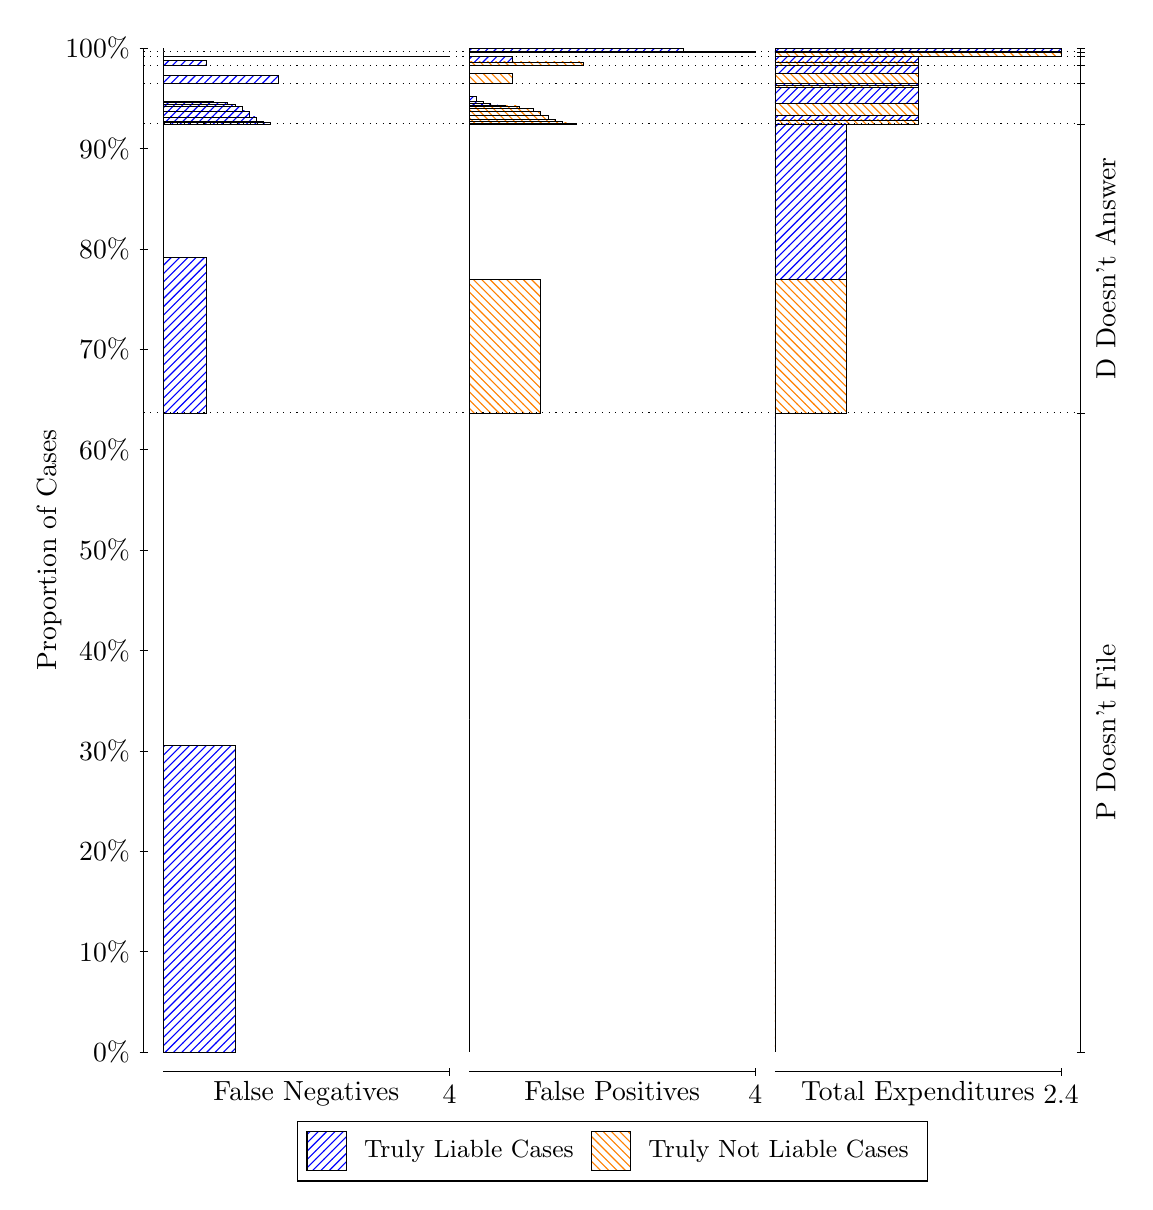
\begin{tikzpicture}
\draw[black, very thin] (1.5,1.75) -- (1.5,14.5);
\node[rotate=90, anchor=center] at (0.3, 8.125) {Proportion of Cases};
\draw[black, very thin] (1.45,1.75) -- (1.55,1.75);
\node[anchor=east] at (1.45, 1.75) {0\%};
\draw[black, very thin] (1.45,3.025) -- (1.55,3.025);
\node[anchor=east] at (1.45, 3.025) {10\%};
\draw[black, very thin] (1.45,4.3) -- (1.55,4.3);
\node[anchor=east] at (1.45, 4.3) {20\%};
\draw[black, very thin] (1.45,5.575) -- (1.55,5.575);
\node[anchor=east] at (1.45, 5.575) {30\%};
\draw[black, very thin] (1.45,6.85) -- (1.55,6.85);
\node[anchor=east] at (1.45, 6.85) {40\%};
\draw[black, very thin] (1.45,8.125) -- (1.55,8.125);
\node[anchor=east] at (1.45, 8.125) {50\%};
\draw[black, very thin] (1.45,9.4) -- (1.55,9.4);
\node[anchor=east] at (1.45, 9.4) {60\%};
\draw[black, very thin] (1.45,10.675) -- (1.55,10.675);
\node[anchor=east] at (1.45, 10.675) {70\%};
\draw[black, very thin] (1.45,11.95) -- (1.55,11.95);
\node[anchor=east] at (1.45, 11.95) {80\%};
\draw[black, very thin] (1.45,13.225) -- (1.55,13.225);
\node[anchor=east] at (1.45, 13.225) {90\%};
\draw[black, very thin] (1.45,14.5) -- (1.55,14.5);
\node[anchor=east] at (1.45, 14.5) {100\%};

\draw[black, very thin] (13.4,1.75) -- (13.4,14.5);
\draw[black, very thin] (13.35,1.75) -- (13.45,1.75);
\node[anchor=west] at (13.35, 1.75) {};
\draw[black, very thin] (13.35,9.8675) -- (13.45,9.8675);
\node[anchor=west] at (13.35, 9.8675) {};
\draw[black, very thin] (13.35,13.536) -- (13.45,13.536);
\node[anchor=west] at (13.35, 13.536) {};
\draw[black, very thin] (13.35,14.046) -- (13.45,14.046);
\node[anchor=west] at (13.35, 14.046) {};
\draw[black, very thin] (13.35,14.281) -- (13.45,14.281);
\node[anchor=west] at (13.35, 14.281) {};
\draw[black, very thin] (13.35,14.389) -- (13.45,14.389);
\node[anchor=west] at (13.35, 14.389) {};
\draw[black, very thin] (13.35,14.452) -- (13.45,14.452);
\node[anchor=west] at (13.35, 14.452) {};
\draw[black, very thin] (13.35,14.5) -- (13.45,14.5);
\node[anchor=west] at (13.35, 14.5) {};

\draw[black, very thin, pattern color=blue, pattern=north east lines] (1.75,1.75) rectangle (2.6583,5.644);
\draw[black, very thin, pattern color=orange, pattern=north west lines] (1.75,5.644) rectangle (1.75,9.8675);
\draw[black, very thin, pattern color=blue, pattern=north east lines] (1.75,9.8675) rectangle (2.295,11.845);
\draw[black, very thin, pattern color=orange, pattern=north west lines] (1.75,11.845) rectangle (1.75,13.536);
\draw[black, very thin, pattern color=blue, pattern=north east lines] (1.75,13.536) rectangle (3.1125,13.555);
\draw[black, very thin, pattern color=blue, pattern=north east lines] (1.75,13.555) rectangle (3.0217,13.567);
\draw[black, very thin, pattern color=blue, pattern=north east lines] (1.75,13.567) rectangle (2.9308,13.626);
\draw[black, very thin, pattern color=blue, pattern=north east lines] (1.75,13.626) rectangle (2.84,13.702);
\draw[black, very thin, pattern color=blue, pattern=north east lines] (1.75,13.702) rectangle (2.7492,13.762);
\draw[black, very thin, pattern color=blue, pattern=north east lines] (1.75,13.762) rectangle (2.6583,13.789);
\draw[black, very thin, pattern color=blue, pattern=north east lines] (1.75,13.789) rectangle (2.5675,13.805);
\draw[black, very thin, pattern color=blue, pattern=north east lines] (1.75,13.805) rectangle (2.4767,13.812);
\draw[black, very thin, pattern color=blue, pattern=north east lines] (1.75,13.812) rectangle (2.3858,13.818);
\draw[black, very thin, pattern color=orange, pattern=north west lines] (1.75,13.818) rectangle (1.75,14.046);
\draw[black, very thin, pattern color=blue, pattern=north east lines] (1.75,14.046) rectangle (3.2033,14.154);
\draw[black, very thin, pattern color=orange, pattern=north west lines] (1.75,14.154) rectangle (1.75,14.281);
\draw[black, very thin, pattern color=blue, pattern=north east lines] (1.75,14.281) rectangle (2.295,14.347);
\draw[black, very thin, pattern color=orange, pattern=north west lines] (1.75,14.347) rectangle (1.75,14.389);
\draw[black, very thin, pattern color=blue, pattern=north east lines] (1.75,14.389) rectangle (5.3833,14.393);
\draw[black, very thin, pattern color=orange, pattern=north west lines] (1.75,14.393) rectangle (1.75,14.452);
\draw[black, very thin, pattern color=orange, pattern=north west lines] (1.75,14.452) rectangle (1.75,14.456);
\draw[black, very thin, pattern color=blue, pattern=north east lines] (1.75,14.456) rectangle (1.75,14.5);
\draw[black, very thin, pattern color=orange, pattern=north west lines] (5.6333,1.75) rectangle (5.6333,5.9735);
\draw[black, very thin, pattern color=blue, pattern=north east lines] (5.6333,5.9735) rectangle (5.6333,9.8675);
\draw[black, very thin, pattern color=orange, pattern=north west lines] (5.6333,9.8675) rectangle (6.5417,11.559);
\draw[black, very thin, pattern color=blue, pattern=north east lines] (5.6333,11.559) rectangle (5.6333,13.536);
\draw[black, very thin, pattern color=orange, pattern=north west lines] (5.6333,13.536) rectangle (6.9958,13.543);
\draw[black, very thin, pattern color=orange, pattern=north west lines] (5.6333,13.543) rectangle (6.905,13.55);
\draw[black, very thin, pattern color=orange, pattern=north west lines] (5.6333,13.55) rectangle (6.8142,13.567);
\draw[black, very thin, pattern color=orange, pattern=north west lines] (5.6333,13.567) rectangle (6.7233,13.595);
\draw[black, very thin, pattern color=orange, pattern=north west lines] (5.6333,13.595) rectangle (6.6325,13.645);
\draw[black, very thin, pattern color=orange, pattern=north west lines] (5.6333,13.645) rectangle (6.5417,13.693);
\draw[black, very thin, pattern color=orange, pattern=north west lines] (5.6333,13.693) rectangle (6.4508,13.73);
\draw[black, very thin, pattern color=orange, pattern=north west lines] (5.6333,13.73) rectangle (6.36,13.738);
\draw[black, very thin, pattern color=orange, pattern=north west lines] (5.6333,13.738) rectangle (6.2692,13.764);
\draw[black, very thin, pattern color=blue, pattern=north east lines] (5.6333,13.764) rectangle (6.0875,13.77);
\draw[black, very thin, pattern color=blue, pattern=north east lines] (5.6333,13.77) rectangle (5.9967,13.777);
\draw[black, very thin, pattern color=blue, pattern=north east lines] (5.6333,13.777) rectangle (5.9058,13.793);
\draw[black, very thin, pattern color=blue, pattern=north east lines] (5.6333,13.793) rectangle (5.815,13.821);
\draw[black, very thin, pattern color=blue, pattern=north east lines] (5.6333,13.821) rectangle (5.7242,13.881);
\draw[black, very thin, pattern color=blue, pattern=north east lines] (5.6333,13.881) rectangle (5.6333,14.046);
\draw[black, very thin, pattern color=orange, pattern=north west lines] (5.6333,14.046) rectangle (6.1783,14.173);
\draw[black, very thin, pattern color=blue, pattern=north east lines] (5.6333,14.173) rectangle (5.6333,14.281);
\draw[black, very thin, pattern color=orange, pattern=north west lines] (5.6333,14.281) rectangle (7.0867,14.324);
\draw[black, very thin, pattern color=blue, pattern=north east lines] (5.6333,14.324) rectangle (6.1783,14.389);
\draw[black, very thin, pattern color=orange, pattern=north west lines] (5.6333,14.389) rectangle (5.6333,14.448);
\draw[black, very thin, pattern color=blue, pattern=north east lines] (5.6333,14.448) rectangle (5.6333,14.452);
\draw[black, very thin, pattern color=orange, pattern=north west lines] (5.6333,14.452) rectangle (9.2667,14.456);
\draw[black, very thin, pattern color=blue, pattern=north east lines] (5.6333,14.456) rectangle (8.3583,14.5);
\draw[black, very thin, pattern color=orange, pattern=north west lines] (9.5167,1.75) rectangle (9.5167,5.9735);
\draw[black, very thin, pattern color=blue, pattern=north east lines] (9.5167,5.9735) rectangle (9.5167,9.8675);
\draw[black, very thin, pattern color=orange, pattern=north west lines] (9.5167,9.8675) rectangle (10.425,11.559);
\draw[black, very thin, pattern color=blue, pattern=north east lines] (9.5167,11.559) rectangle (10.425,13.536);
\draw[black, very thin, pattern color=orange, pattern=north west lines] (9.5167,13.536) rectangle (11.333,13.586);
\draw[black, very thin, pattern color=blue, pattern=north east lines] (9.5167,13.586) rectangle (11.333,13.646);
\draw[black, very thin, pattern color=orange, pattern=north west lines] (9.5167,13.646) rectangle (11.333,13.8);
\draw[black, very thin, pattern color=blue, pattern=north east lines] (9.5167,13.8) rectangle (11.333,13.999);
\draw[black, very thin, pattern color=orange, pattern=north west lines] (9.5167,13.999) rectangle (11.333,14.023);
\draw[black, very thin, pattern color=blue, pattern=north east lines] (9.5167,14.023) rectangle (11.333,14.046);
\draw[black, very thin, pattern color=orange, pattern=north west lines] (9.5167,14.046) rectangle (11.333,14.173);
\draw[black, very thin, pattern color=blue, pattern=north east lines] (9.5167,14.173) rectangle (11.333,14.281);
\draw[black, very thin, pattern color=orange, pattern=north west lines] (9.5167,14.281) rectangle (11.333,14.324);
\draw[black, very thin, pattern color=blue, pattern=north east lines] (9.5167,14.324) rectangle (11.333,14.389);
\draw[black, very thin, pattern color=orange, pattern=north west lines] (9.5167,14.389) rectangle (13.15,14.448);
\draw[black, very thin, pattern color=blue, pattern=north east lines] (9.5167,14.448) rectangle (13.15,14.452);
\draw[black, very thin, pattern color=orange, pattern=north west lines] (9.5167,14.452) rectangle (13.15,14.456);
\draw[black, very thin, pattern color=blue, pattern=north east lines] (9.5167,14.456) rectangle (13.15,14.5);
\draw[black, dotted] (1.5,9.8675) -- (13.4,9.8675);
\draw[black, dotted] (1.5,13.536) -- (13.4,13.536);
\draw[black, dotted] (1.5,14.046) -- (13.4,14.046);
\draw[black, dotted] (1.5,14.281) -- (13.4,14.281);
\draw[black, dotted] (1.5,14.389) -- (13.4,14.389);
\draw[black, dotted] (1.5,14.452) -- (13.4,14.452);
\draw[black, very thin] (1.75,1.5) -- (5.3833,1.5);
\node[anchor=north] at (3.5667, 1.5) {False Negatives};
\draw[black, very thin] (5.3833,1.45) -- (5.3833,1.55);
\node[anchor=north] at (5.3833, 1.45) {4};

\draw[black, very thin] (5.6333,1.5) -- (9.2667,1.5);
\node[anchor=north] at (7.45, 1.5) {False Positives};
\draw[black, very thin] (9.2667,1.45) -- (9.2667,1.55);
\node[anchor=north] at (9.2667, 1.45) {4};

\draw[black, very thin] (9.5167,1.5) -- (13.15,1.5);
\node[anchor=north] at (11.333, 1.5) {Total Expenditures};
\draw[black, very thin] (13.15,1.45) -- (13.15,1.55);
\node[anchor=north] at (13.15, 1.45) {2.4};

\node[black, centered, rotate=90] at (13.72, 5.8087) {P Doesn't File};
\node[black, centered, rotate=90] at (13.72, 11.702) {D Doesn't Answer};






\draw (7.449999999999999,1.5) node[draw=none] (baseCoordinate) {};
\begin{scope}[align=center]
        \matrix[scale=0.5, draw=black, below=0.5cm of baseCoordinate, nodes={draw}, column sep=0.1cm]{
            \node[rectangle, draw, minimum width=0.5cm, minimum height=0.5cm, pattern=north east lines, pattern color=blue] {}; &
            \node[draw=none, font=\small] (B) {Truly Liable Cases}; &
            \node[rectangle, draw, minimum width=0.5cm, minimum height=0.5cm, pattern=north west lines, pattern color=orange] {}; &
            \node[draw=none, font=\small] (B) {Truly Not Liable Cases}; \\
            };
\end{scope}

\end{tikzpicture}
\end{document}